\chapter{Testing}

\section{Website}

First, the website is tested. The program on the second core is modified for the purpose of testing. Instead of correctly filtering the input its more important task will be periodically logging the value of alpha and beta to the serial line, even if it interferes with the timing of the DAC module.

\begin{figure}[H]
    \centering
    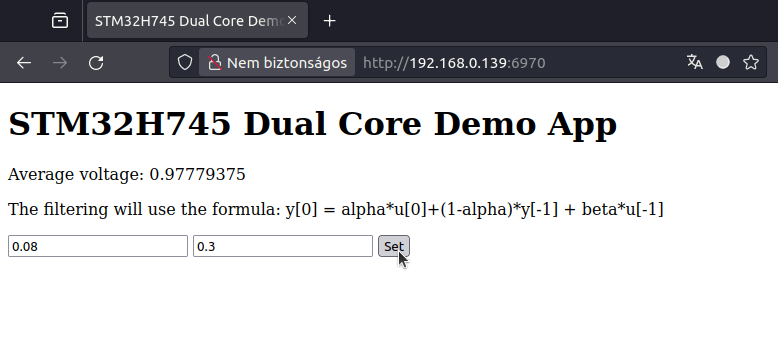
\includegraphics[width=150mm, keepaspectratio]{figures/webpage-test1.png}
    \caption{Webpage Before Inputting New Coefficients}
    \label{fig:webpage-test1}
\end{figure}

Inputting new values on the webpage to this modified program results in the following output on a terminal monitoring the serial port.

\begin{figure}[H]
    \centering
    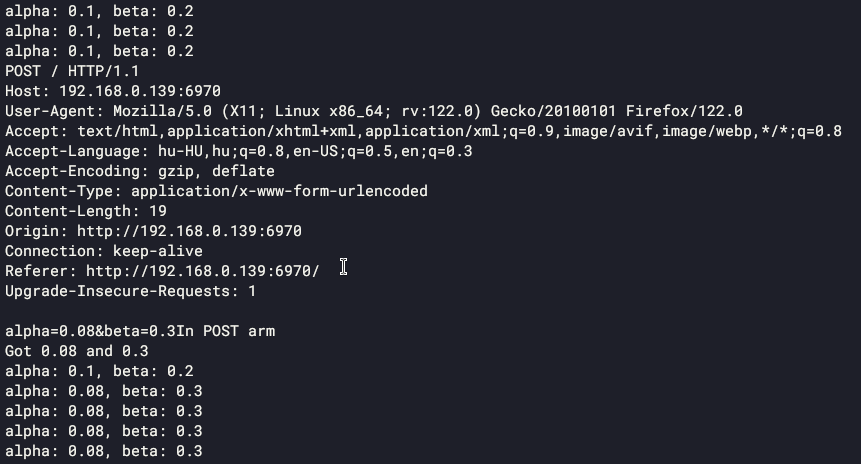
\includegraphics[width=150mm, keepaspectratio]{figures/coef-log.png}
    \caption{Serial Output when New Coefficients Are Supplied}
    \label{fig:coef-log}
\end{figure}

Supplying new variables refreshes the site, which is currently the only way to change the average voltage displayed. During the test, a sine wave with an amplitude of 500 mv and an offset of 1 V was supplied to the ADC.

\begin{figure}[H]
    \centering
    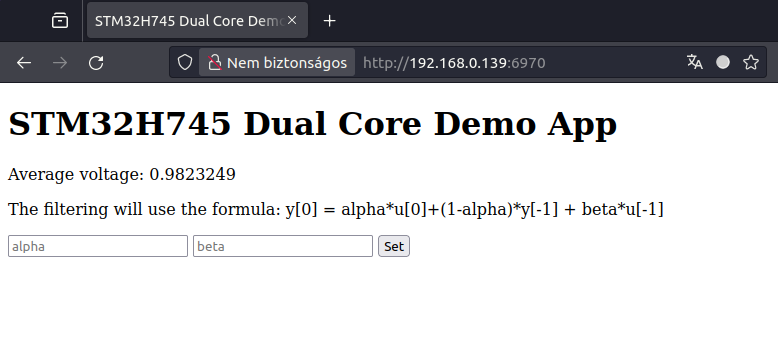
\includegraphics[width=150mm, keepaspectratio]{figures/webpage-test2.png}
    \caption{Webpage With Changed Average Voltage}
    \label{fig:webpage-test2}
\end{figure}

These results confirm that the two cores can communicate and exchange the necessary data. Also that the website works correctly is confirmed too.

\section{Low Pass Filter}

\subsection{DAC Capabilities}

Testing the functionality of the second core required a tool that can generate an input and handle the output of the analog peripherals on the microcontroller. For this purpose, a Picoscope 2000 series oscilloscope was used. It can act as a traditional digital oscilloscope and also generate arbitrary functions either based on common signals or a series of samples.

As a first step, I wanted to figure out the maximum frequency of the DAC using this configuration in the worst case scenario. I used code on the M4 core that alternates the DAC output between the minimum and the maximum value. As Figure~{fig:dac-timing} suggests, we will need to leave time for the DAC to settle after requesting a change on its output. In theory, this time equals 3 bus cycles. The AHB bus frequency matches the system clock frequency, 200 MHz in this case. In practice however I have found that at least 15 cycles are needed for the DAC to settle. This is most likely due to other overheads during the usage of the peripheral.

\begin{lstlisting}[language=Rust,frame=single,float=!ht,style=customrust,label={lst:only-dac-test},caption={Code for Testing DAC Frequency Limit}]
    let mut nops: u32 = 15;
    loop {
        dac.set_value(0);
        for i in 0..nops {
            cortex_m::asm::nop();
        }
        dac.set_value(4095);
        for i in 0..nops {
            cortex_m::asm::nop();
        }
    }
\end{lstlisting}

In Listing~\ref{lst:only-dac-test} the \mycode{cortex::asm::nop()} function is used to force a \mycode{nop} instruction. Using this method prevents the compiler from optimizing this seemingly unnecessary wait period.

The figure below shows that 15 cycles were needed for the best results in this test case. The frequency was measured at around 300 kHz, so this is the theoretical maximum that can be achieved using this method to control the DAC and assuming worst case output changes.

\begin{figure}[H]
    \centering
    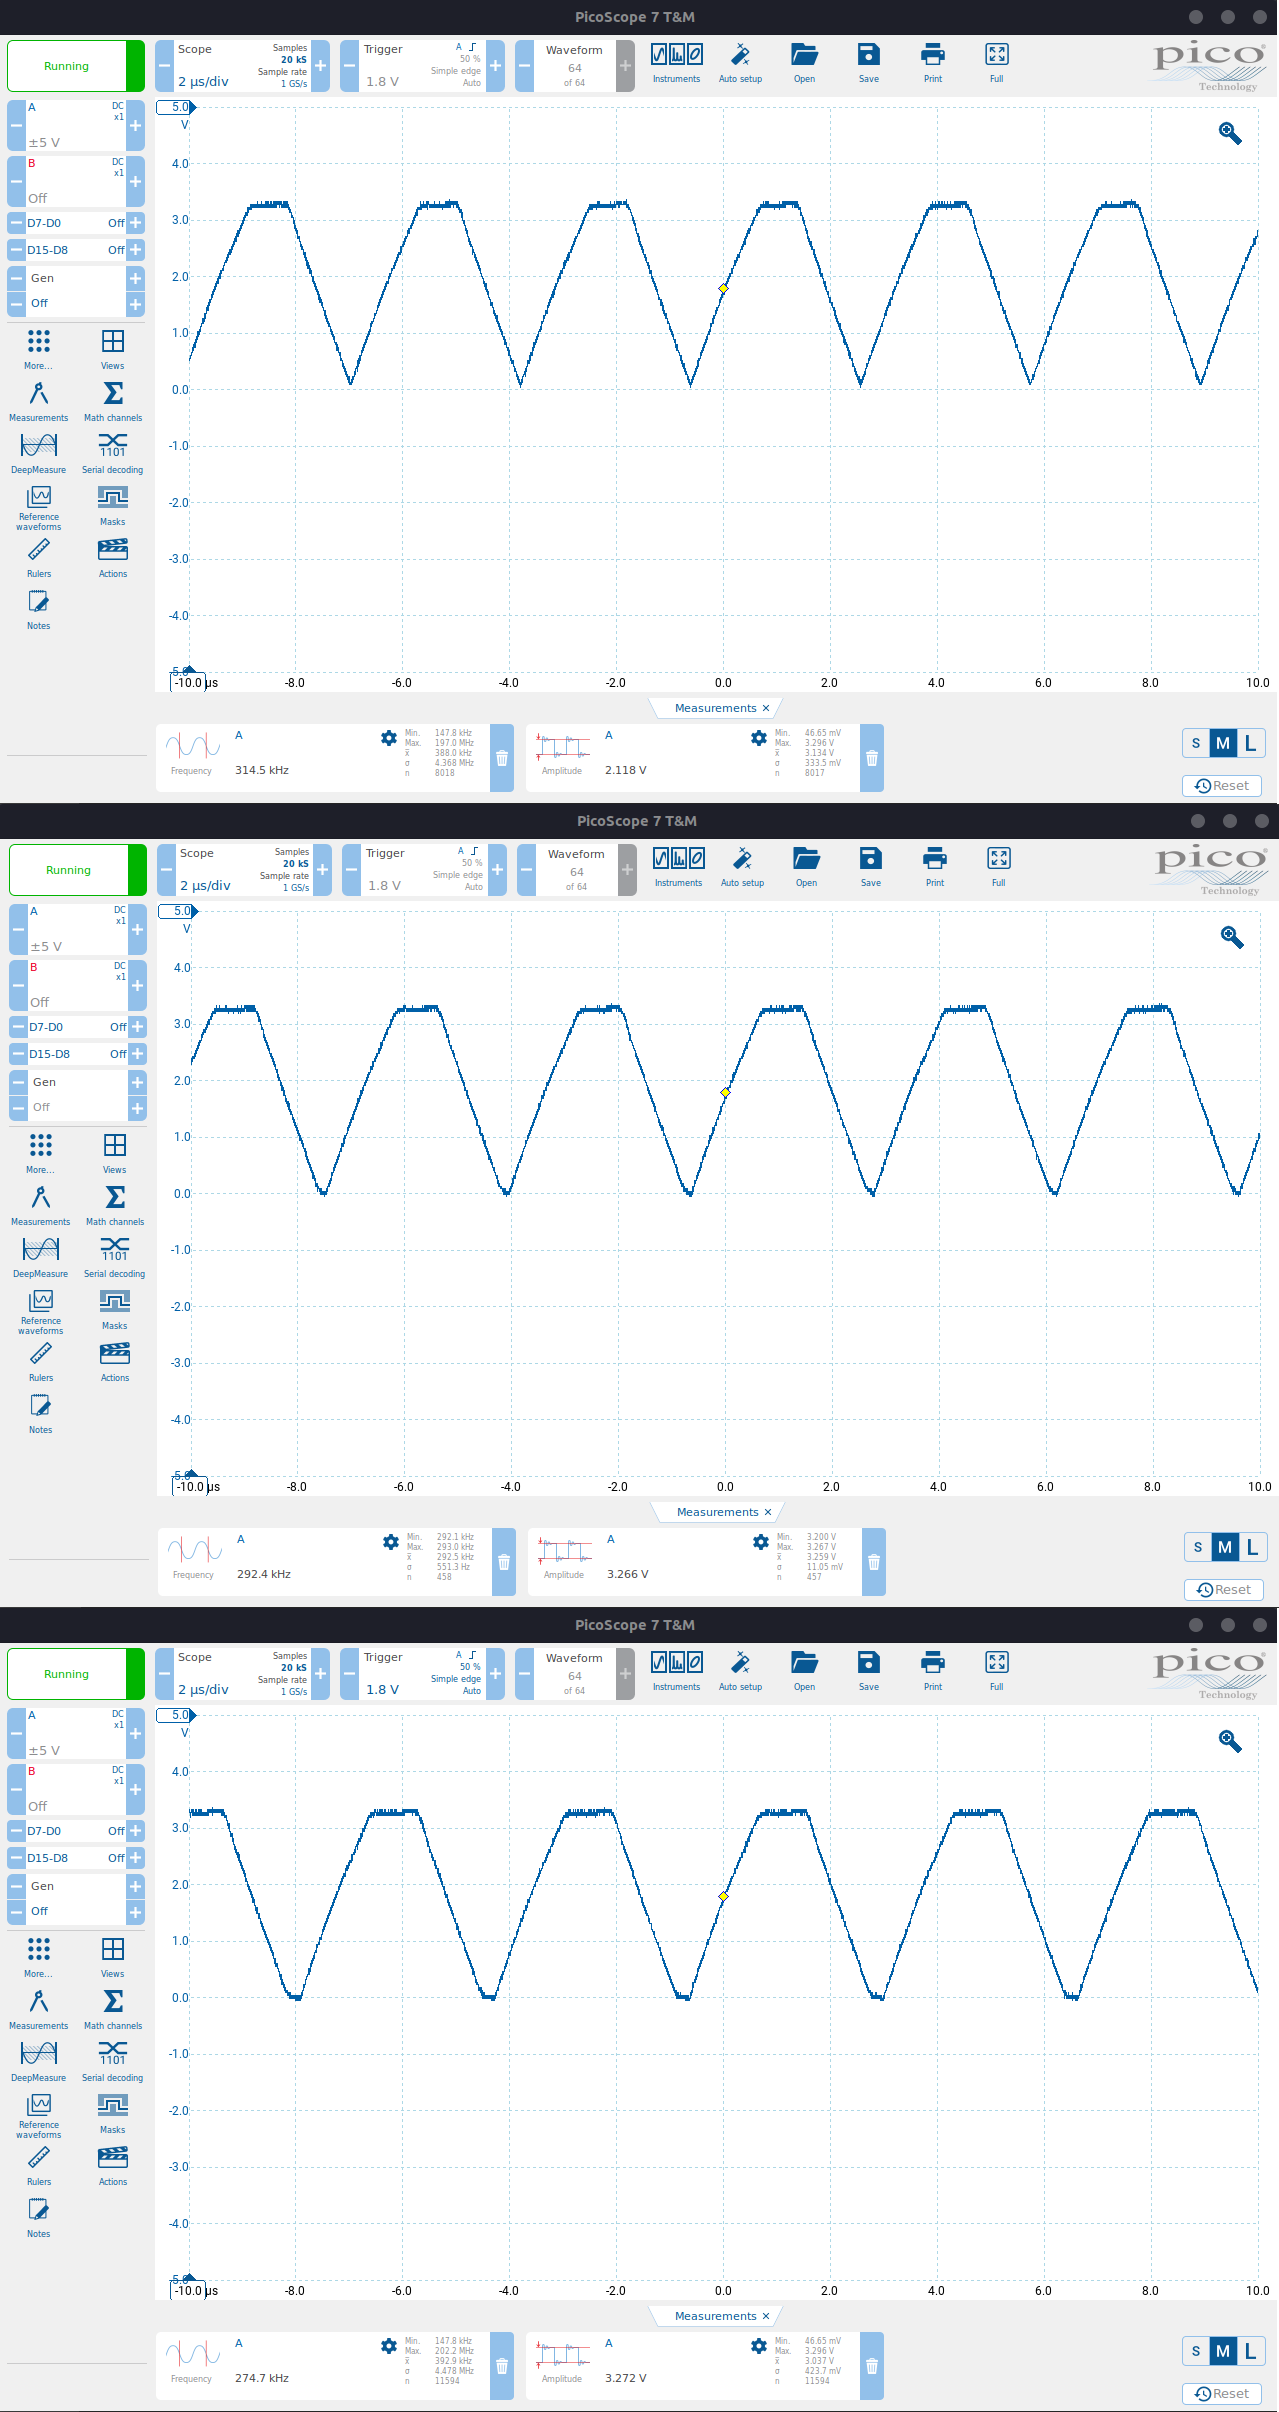
\includegraphics[width=120mm, keepaspectratio]{figures/comp.png}
    \caption{Output with 14, 15, and 16 \mycode{nop()}s Respectively}
    \label{fig:comp}
\end{figure}

\subsection{ADC Capabilities}

Handling the ADC and waiting for a conversion makes up for the 15 cycles needed for the DAC to settle. As a blocking call to the ADC is made to get a sample, the \mycode{nop()} calls can be removed entirely. In this test, the microcontroller samples its analog input, and outputs the same value on its analog output.

\begin{lstlisting}[language=Rust,frame=single,float=!ht,style=customrust,label={lst:adc-dac-test},caption={Code for Testing ADC and DAC Together}]
    loop {
        let reading: u32 = adc1.read(&mut channel).unwrap();
        let output: u16 = (reading as f32 / 16.0) as u16;
        dac.set_value(output);
    }
\end{lstlisting}

The highest frequency in this case was around 20 kHz. At higher frequency values the dampening of the system was above 10\%. Despite the loss of magnitude, the signal could be recognized as a sine wave even at 50 kHz.

\begin{figure}[H]
    \centering
    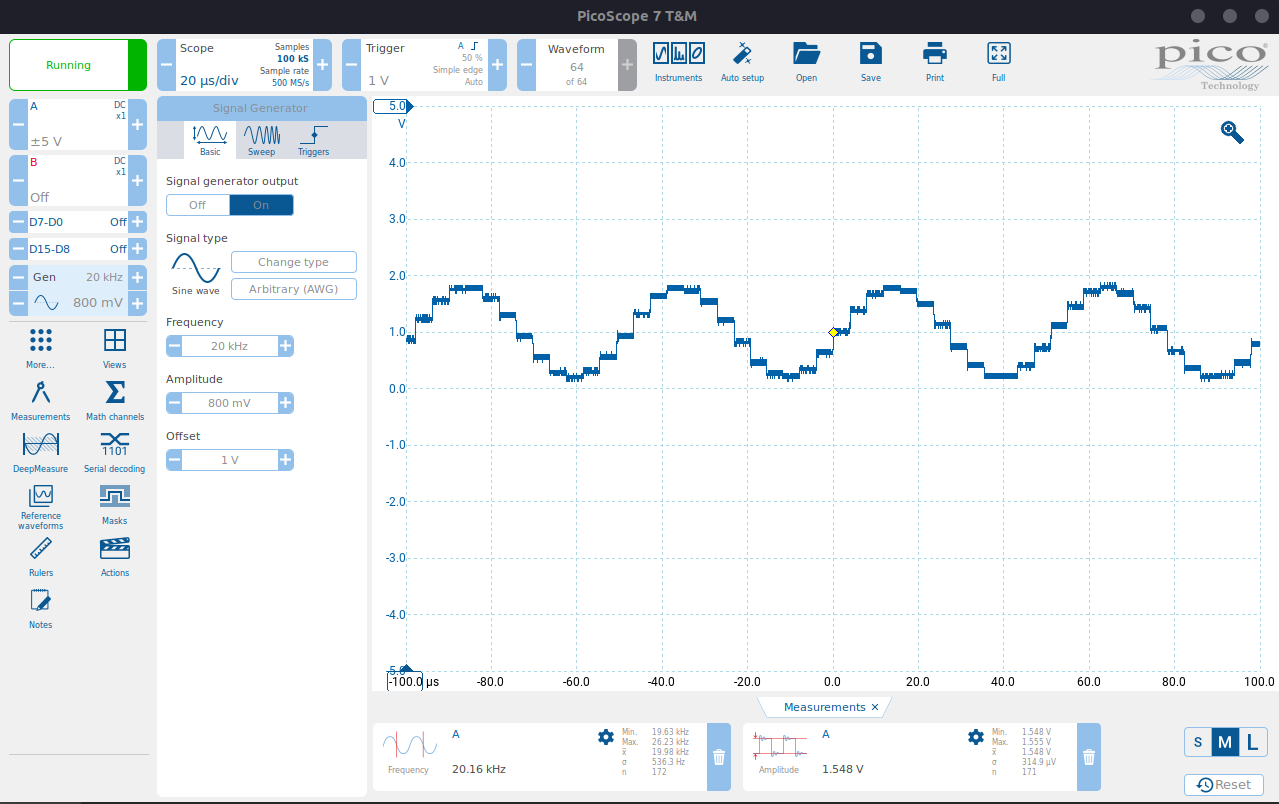
\includegraphics[width=150mm, keepaspectratio]{figures/sine20khz.png}
    \caption{Output at 20 kHz}
    \label{fig:sine20khz}
\end{figure}

\subsection{Filter Capabilities}

In this section, the code used already contains the implemented filter. The first step in this test was to plot the expected Bode diagrams of the filter with some configurations.

\begin{figure}[H]
    \centering
    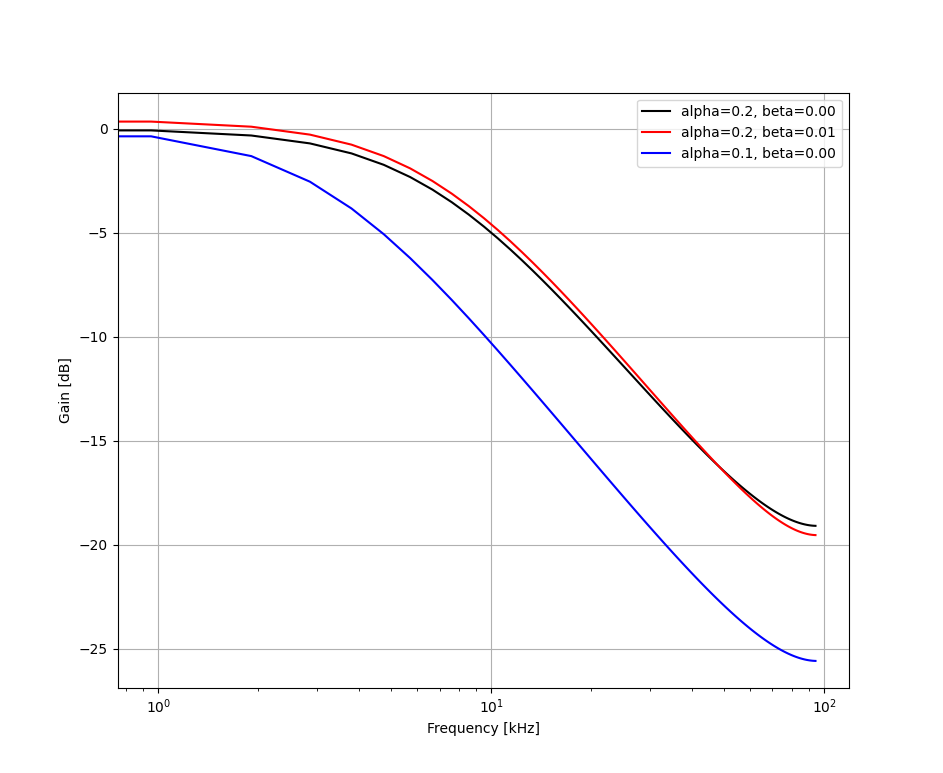
\includegraphics[width=150mm, keepaspectratio]{figures/bode.png}
    \caption{Bode Diagram of the Filter with Various Parameters}
    \label{fig:bode}
\end{figure}

Based on this diagram, \mycode{alpha = 0.2} will be used for further experiments as it provides a higher cutoff frequency thus a wider buffer range.

I measured the gain in the cases where \mycode{alpha = 0.2}, and found that the previous simulation is a good approximation of the real filter.

\begin{figure}[H]
    \centering
    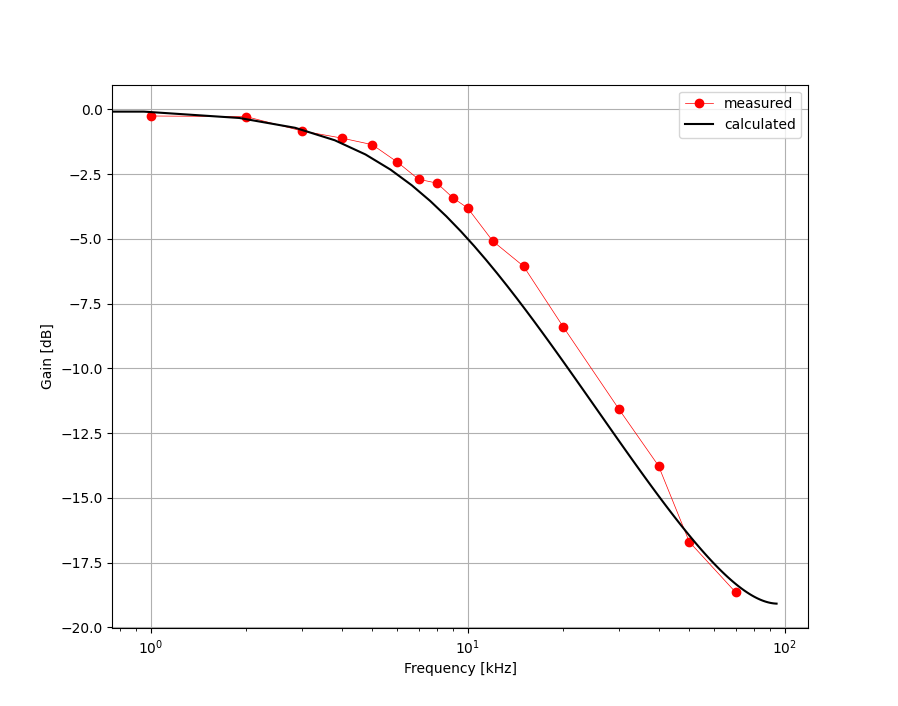
\includegraphics[width=150mm, keepaspectratio]{figures/bode02000.png}
    \caption{Gain at Various Frequencies \mycode{alpha = 0.2} and \mycode{beta = 0}}
    \label{fig:bode02000}
\end{figure}

\begin{table}[H]
    \centering
    \begin{tabular}{cc}
        \hline
        \textbf{Frequency [kHz]} & \textbf{Amplitude [V]} \\
        \hline
        1   & 1.554 \\
        2   & 1.550 \\
        3   & 1.454 \\
        4   & 1.409 \\
        5   & 1.368 \\
        6   & 1.266 \\
        7   & 1.173 \\
        8   & 1.153 \\
        9   & 1.079 \\
        10  & 1.032 \\
        12  & 0.891 \\
        15  & 0.797 \\
        20  & 0.609 \\
        30  & 0.422 \\
        40  & 0.328 \\
        50  & 0.234 \\
        70  & 0.187 \\
        \hline
    \end{tabular}
    \caption{Frequency and Amplitude \mycode{alpha = 0.2} and \mycode{beta = 0}}
    \label{tab:freq_mag_data}
\end{table}

\begin{figure}[H]
    \centering
    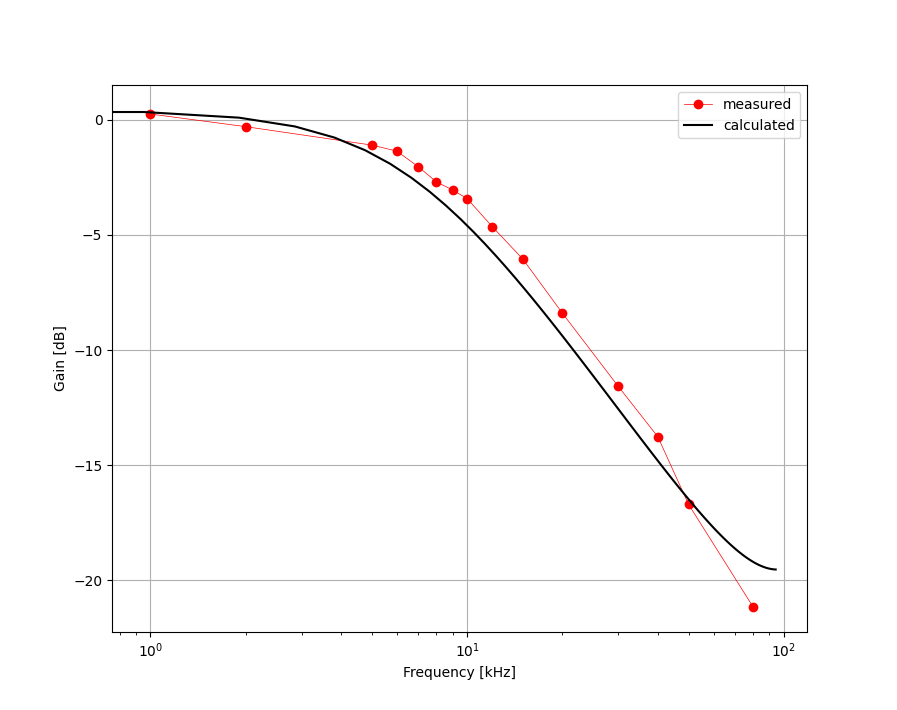
\includegraphics[width=150mm, keepaspectratio]{figures/bode02001.png}
    \caption{Gain at Various Frequencies \mycode{alpha = 0.2} and \mycode{beta = 0.01}}
    \label{fig:bode02001}
\end{figure}

\begin{table}[htbp]
    \centering
    \begin{tabular}{cc}
        \hline
        \textbf{Frequency [kHz]} & \textbf{Voltage [V]} \\
        \hline
        1   & 1.647 \\
        2   & 1.546 \\
        5   & 1.410 \\
        6   & 1.368 \\
        7   & 1.266 \\
        8   & 1.173 \\
        9   & 1.126 \\
        10  & 1.079 \\
        12  & 0.938 \\
        15  & 0.797 \\
        20  & 0.608 \\
        30  & 0.422 \\
        40  & 0.328 \\
        50  & 0.234 \\
        80  & 0.140 \\
        \hline
    \end{tabular}
    \caption{Frequency and Voltage \mycode{alpha = 0.2} and \mycode{beta = 0.01}}
    \label{tab:freq_mag_data_2}
\end{table}

Finally, I tested the filtering capabilities of this system with a noisy input. I created the input by adding white noise to a sine wave.

\begin{figure}[H]
    \centering
    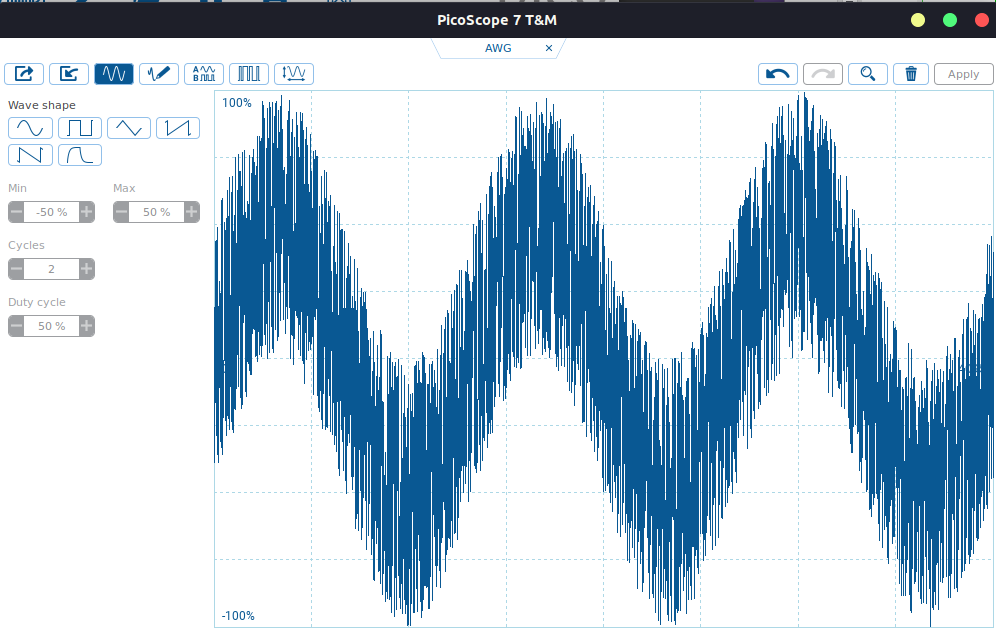
\includegraphics[width=150mm, keepaspectratio]{figures/sineerror.png}
    \caption{Sine Wave with Added Noise}
    \label{fig:sineerror}
\end{figure}

This signal can be used as the output of the Picoscope used for testing. The scope can modify the frequency and amplitude of this signal. For this test, the \mycode{alpha = 0.2} and \mycode{beta = 0.01} configuration was used. The dampening at with this signal started at lower frequencies. At 100 Hz a fairly clear sine wave can be observed, and this remains the case up until 4 kHz.

\begin{figure}[H]
    \centering
    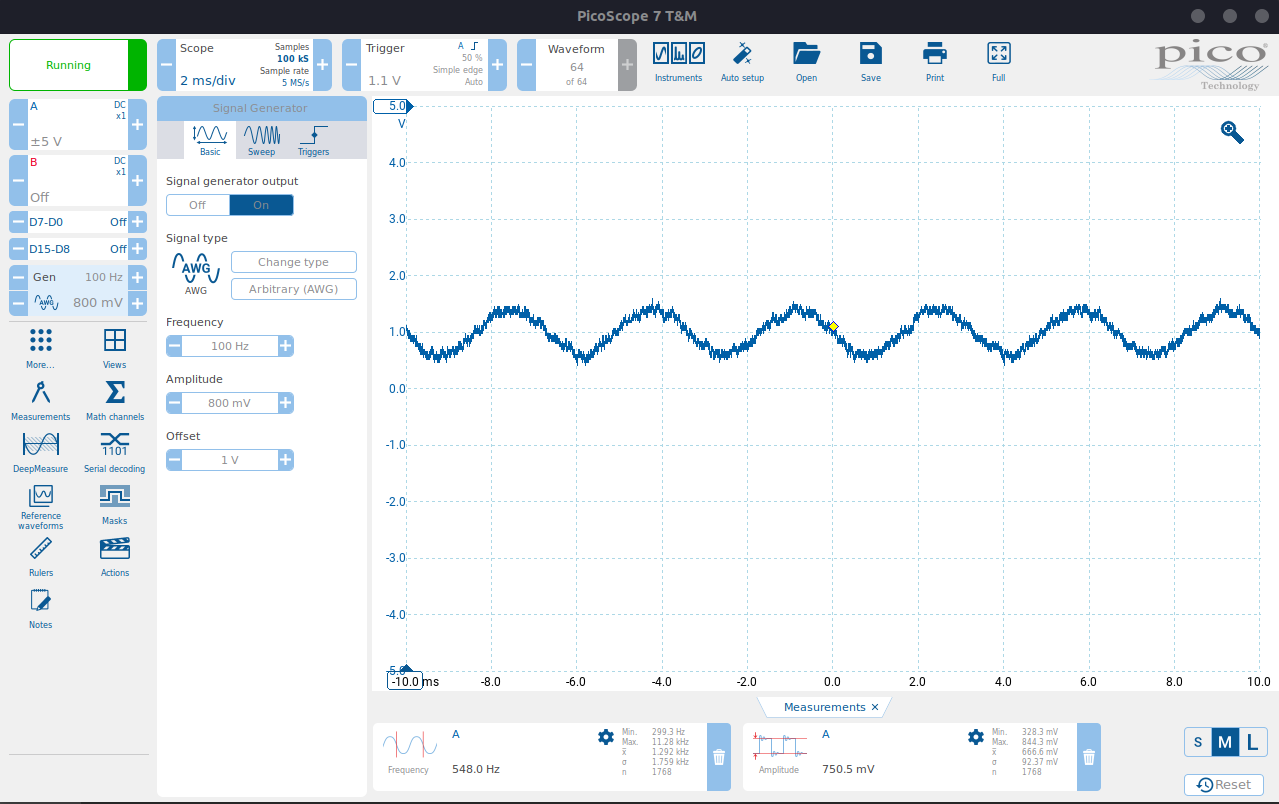
\includegraphics[width=150mm, keepaspectratio]{figures/filter100.png}
    \caption{Filtered Noisy Sine Wave at 100 Hz}
    \label{fig:filter100}
\end{figure}

\begin{figure}[H]
    \centering
    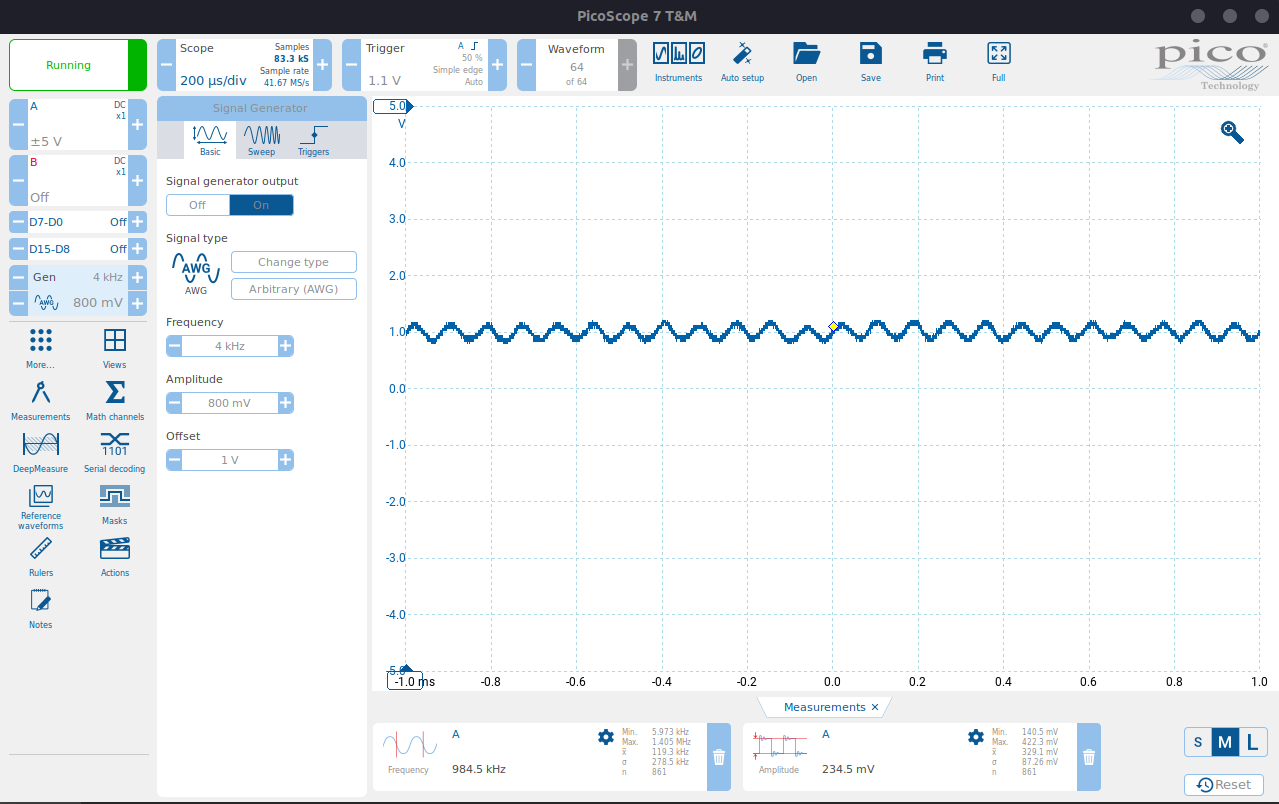
\includegraphics[width=150mm, keepaspectratio]{figures/filter4.png}
    \caption{Filtered Noisy Sine Wave at 4 kHz}
    \label{fig:filter4}
\end{figure}

Raising the frequency any higher results in too much dampening, so the output cannot be interpreted as a sine wave.

\begin{figure}[H]
    \centering
    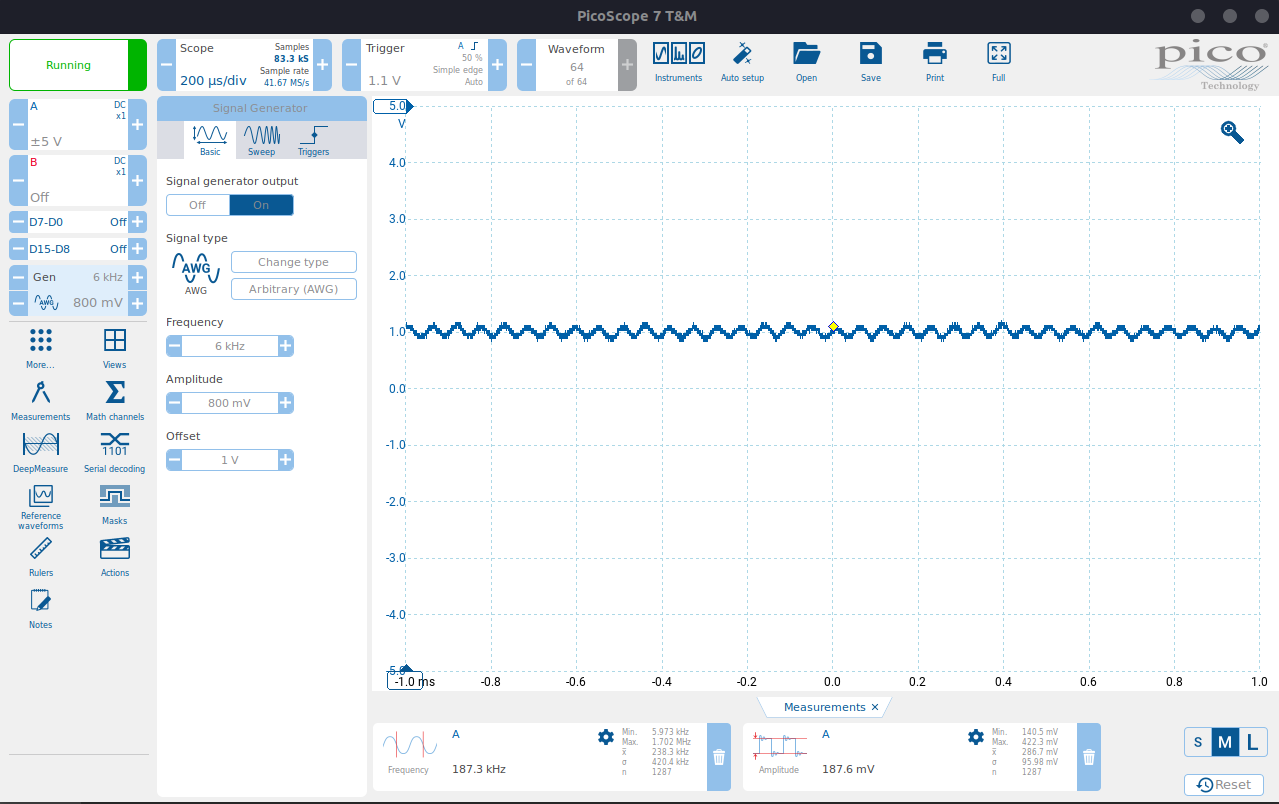
\includegraphics[width=150mm, keepaspectratio]{figures/filter6.png}
    \caption{Filtered Noisy Sine Wave at 6 kHz}
    \label{fig:filter6}
\end{figure}
